%==========================================================================
% Exemplo de artigo cientifico UNESC
%
% v0.0 versão em 20/09/2023 por Marlon Oliveira
% v1.0 versão em 25/06/2025 por Marlon Oliveira


%==========================================================================

%==========================================================================
% Pacotes utilizados pela UNESC - não delete as linhas abaixo
%==========================================================================
\documentclass{UNESC}
\usepackage[T1]{fontenc}
\usepackage[utf8]{inputenc}%\usepackage[latin1]{inputenc}
\renewcommand{\rmdefault}{phv} % Arial
\renewcommand{\sfdefault}{phv} % Arial
\usepackage[brazilian]{babel}
\usepackage{graphicx}
%\usepackage{subfigure}
\usepackage{hyperref}
\usepackage{quoting}
\usepackage[labelsep=none]{caption}
\DeclareCaptionLabelFormat{figuracomtraco}{#1~#2 -}
\captionsetup[figure]{labelformat=figuracomtraco, labelsep=space}
\captionsetup[table]{labelformat=simple, labelsep=space, textformat=simple}
\DeclareCaptionLabelFormat{tabelacomtraco}{#1~#2 -}
\captionsetup[table]{labelformat=tabelacomtraco}
\captionsetup{labelsep=none}
%\renewcommand{\thefigure}{\arabic{figure} - }
\usepackage{enumitem}
\usepackage{float}
\usepackage{comment}
\usepackage[hang,flushmargin]{footmisc}
\usepackage{array}
% Pacotes adicionais para os quadros e o fluxograma solicitados na revisão.
\usepackage{booktabs}
\usepackage{tabularx}
\usepackage{longtable}
\usepackage{tikz}
\usetikzlibrary{arrows.meta,positioning}
\usepackage{amsmath}
\usepackage{listings}
\usepackage{placeins}
\newcolumntype{Y}{>{\raggedright\arraybackslash}X}
\newcommand{\fonteautor}{\par\smallskip{\footnotesize Fonte: elaboração própria.}}
\lstset{basicstyle=\ttfamily\footnotesize,breaklines=true,columns=fullflexible,
  frame=single,showstringspaces=false,keepspaces=true}
\setlength{\emergencystretch}{2em}

\hypersetup{
  setpagesize  = false,
  colorlinks   = true,    % Colours links instead of ugly boxes
  urlcolor     = blue,    % Colour for external hyperlinks
  linkcolor    = black,   % Colour of internal links
  citecolor    = black    % Colour of citations
}
\urlstyle{same}
\usepackage{setspace}

\usepackage[alf,recuo=0.0cm,abnt-emphasize=bf]{abntex2cite} 

%\captionsetup[figure]{justification=raggedright}



%==========================================================================
% Dados do artigo: título, autores e filiação
%==========================================================================
\title{ANÁLISE E OTIMIZAÇÃO DE CONSULTAS SQL COM BASE EM LOGS DE EXECUÇÃO EM BANCOS DE DADOS RELACIONAIS}

\author
{
   Arthur Meira\footnote{Curso de Ciência da Computação, Universidade do Extremo Sul Catarinense (Unesc), Criciúma - Santa Catarina - Brasil. arthurmeiraprog@unesc.net},
   Marcel Campos Inocencio\footnote{Orientador, Curso de Ciência da Computação, Universidade do Extremo Sul Catarinense (Unesc), Criciúma - Santa Catarina - Brasil. marcel.inocencio@gmail.com}
}

%==========================================================================
% Início do texto do artigo
%==========================================================================
\begin{document}

\onehalfspacing

\maketitle

%==========================================================================
% Resumo e abstract atualizados com os resultados documentados.
%==========================================================================

\noindent
\textbf{Resumo:} Consultas SQL lentas podem gerar gargalos e comprometer o desempenho de sistemas que utilizam bancos de dados relacionais. Este trabalho teve como objetivo desenvolver uma ferramenta para auxiliar na identificação e na análise preventiva de consultas com possíveis problemas de desempenho. Para avaliar a solução, foi criado um banco de dados experimental com informações fictícias de clientes, produtos, pedidos, itens e pagamentos, totalizando 4.648.714 registros. Em seguida, foi executado um conjunto de consultas com diferentes características e frequências de utilização. As informações sobre essas execuções foram coletadas no PostgreSQL e combinadas com a análise dos planos de execução. A ferramenta desenvolvida identifica sinais como varreduras sequenciais em tabelas grandes, funções aplicadas em filtros, respostas com muitas linhas e diferenças entre a quantidade estimada e a quantidade histórica de registros. Os resultados permitiram localizar consultas com elevado tempo de execução e avaliar possíveis alterações em sua escrita. Em um dos experimentos, a substituição de uma função aplicada sobre uma coluna indexada permitiu que o banco utilizasse o índice existente. Nas condições avaliadas, essa alteração reduziu o tempo médio de execução no servidor de 26,33 para 0,0303 milissegundo, mantendo o mesmo resultado. Também foi desenvolvida uma interface web para apresentar as consultas, os planos, os sinais encontrados e as sugestões de melhoria. Concluiu-se que a combinação de estatísticas históricas, planos de execução e regras explicáveis pode auxiliar na investigação de consultas lentas, desde que as alterações sugeridas sejam confirmadas por testes de equivalência e desempenho.

\vspace{0.5em}
\noindent
\textbf{Palavras-chave:} bancos de dados relacionais; consultas SQL; otimização de consultas; estatísticas de execução; planos de execução.

\vspace{1.0em}
\noindent
\textbf{ABSTRACT:} Slow SQL queries can create bottlenecks and affect the performance of systems that use relational databases. This study aimed to develop a tool to assist in the identification and preventive analysis of queries with possible performance problems. To evaluate the solution, an experimental database containing fictional data about customers, products, orders, order items, and payments was created, totaling 4,648,714 records. A set of queries with different characteristics and execution frequencies was then performed. Information about these executions was collected from PostgreSQL and combined with the analysis of execution plans. The developed tool identifies warning signs such as sequential scans on large tables, functions applied to filters, queries that return a large number of rows, and differences between the estimated and historical number of records. The results made it possible to identify queries with high execution times and evaluate possible changes to their SQL statements. In one experiment, removing a function applied to an indexed column allowed the database to use the existing index. Under the evaluated conditions, this change reduced the mean server execution time from 26.33 to 0.0303 milliseconds while preserving the same result. A web interface was also developed to present the queries, execution plans, detected warning signs, and improvement suggestions. It was concluded that combining historical statistics, execution plans, and explainable rules can support the investigation of slow queries, provided that the suggested changes are confirmed through equivalence and performance tests.

\vspace{0.5em}
\noindent
\textbf{Keywords:} relational databases; SQL queries; query optimization; execution statistics; execution plans.
%==========================================================================
% Introdução
%==========================================================================

\section{INTRODUÇÃO}

A linguagem SQL (\textit{Structured Query Language}) é utilizada para consultar e manipular informações armazenadas em bancos de dados relacionais. Ao escrever uma consulta, o desenvolvedor informa quais dados deseja obter, enquanto o sistema gerenciador de banco de dados (SGBD) determina como essa busca será realizada. Uma mesma consulta pode ser executada de diferentes formas, dependendo da quantidade de dados, dos índices disponíveis, dos filtros aplicados e das operações necessárias para produzir o resultado \cite{lan2021optimizer}.

A escolha da forma de execução é realizada pelo otimizador de consultas. Esse componente analisa diferentes possibilidades e seleciona um plano de execução. O plano apresenta as operações que o banco pretende realizar, como a leitura de tabelas, a aplicação de filtros, as junções, os agrupamentos e as ordenações. Mesmo quando duas estratégias retornam os mesmos dados, elas podem apresentar diferenças significativas no uso de recursos e no tempo necessário para concluir a consulta.

De acordo com \citeonline{lan2021optimizer}, a escolha de um plano depende principalmente da estimativa da quantidade de registros, do cálculo do custo das operações e da análise das alternativas disponíveis. A estimativa da quantidade de registros, também chamada de estimativa de cardinalidade, indica quantas linhas cada etapa do plano deve produzir. Quando essa previsão se distancia da quantidade real, o banco pode escolher uma estratégia menos adequada.

As características dos dados também influenciam esse processo. \citeonline{kossmann2022dependencies} discutem como restrições de unicidade e dependências entre atributos podem apoiar a otimização. Uma coluna sem valores repetidos, por exemplo, fornece uma informação diferente daquela que permite várias ocorrências do mesmo valor. Conhecer essas propriedades pode permitir simplificar operações, desde que as condições necessárias sejam válidas no conjunto analisado. Uma alteração baseada em uma suposição incorreta pode modificar o resultado esperado da consulta.

Além da análise do plano, é necessário observar o comportamento das consultas ao longo do uso do banco de dados. Uma consulta lenta executada poucas vezes possui um impacto diferente de uma consulta mais rápida que se repete milhares de vezes. Estatísticas como quantidade de chamadas, tempo total, tempo médio e número de linhas retornadas ajudam a identificar quais consultas merecem ser investigadas primeiro.

A análise de desempenho geralmente exige conhecimento técnico para interpretar essas informações. Uma varredura sequencial, por exemplo, não representa necessariamente um problema, pois pode ser adequada quando a consulta retorna grande parte de uma tabela. Da mesma forma, a criação de um índice não garante melhoria e pode aumentar o custo das operações de inserção e atualização. Por isso, as recomendações precisam ser apresentadas como possibilidades que devem ser verificadas por meio de testes.

A pesquisa se justifica pela necessidade de identificar e reduzir gargalos provocados por consultas SQL lentas. Esses gargalos podem aumentar o tempo de resposta das aplicações, elevar o consumo de recursos do servidor e prejudicar vários usuários ao mesmo tempo. Sem um processo de análise, alterações podem ser aplicadas sem evidências suficientes ou consultas de baixo impacto podem receber prioridade enquanto problemas mais relevantes permanecem sem investigação.

Diante desse contexto, esta pesquisa busca responder à seguinte questão: como combinar estatísticas históricas e planos de execução para identificar consultas SQL potencialmente problemáticas, explicar os sinais encontrados e apoiar a validação de melhorias em bancos de dados relacionais?

O objetivo geral é desenvolver e avaliar um processo automatizado de análise preventiva de consultas SQL baseado em estatísticas históricas e planos de execução. Os objetivos específicos são construir uma base experimental reprodutível, executar consultas com diferentes características, coletar e classificar suas métricas, identificar possíveis problemas nos planos, comparar consultas originais e alternativas, validar o efeito das alterações e apresentar as informações em uma interface visual.

A principal contribuição deste trabalho está na integração dessas etapas em uma ferramenta de apoio. A solução não aplica alterações automaticamente e não substitui a avaliação de um especialista. Seu propósito é reunir as evidências encontradas, explicar por que uma consulta recebeu determinado nível de atenção e auxiliar na decisão sobre quais mudanças devem ser testadas.



% Corpo simplificado, mantido próximo ao texto corrigido pelo professor.
\section{MATERIAIS E MÉTODOS}

Iniciou-se a parte prática com a construção de um protótipo capaz de executar consultas SQL, coletar informações sobre essas execuções e apresentar possíveis pontos de atenção. O estudo foi realizado em um ambiente controlado, com dados fictícios, para que os testes não interferissem em um sistema real.

O trabalho foi organizado em seis etapas. Primeiro, construiu-se o banco experimental. Depois, geraram-se e carregaram-se os dados. Na terceira etapa, executou-se um conjunto de consultas para formar um histórico. Na quarta, coletaram-se as estatísticas e selecionaram-se as consultas mais relevantes. Na quinta, analisaram-se os planos de execução. Por fim, comparou-se uma alteração de consulta e verificou-se seu resultado. A Figura~\ref{fig:fluxo-simples} apresenta esse processo.

\begin{figure}[H]
\centering
\caption{Etapas da solução desenvolvida}
\label{fig:fluxo-simples}
\begin{tikzpicture}[
etapa/.style={rectangle,draw=black,rounded corners,align=center,
  text width=10.5cm,minimum height=0.78cm,font=\small},
seta/.style={-{Latex[length=2mm]},thick},node distance=0.35cm]
\node[etapa] (e1) {1. Construção do banco experimental};
\node[etapa,below=of e1] (e2) {2. Geração e carregamento dos dados fictícios};
\node[etapa,below=of e2] (e3) {3. Execução das consultas e formação do histórico};
\node[etapa,below=of e3] (e4) {4. Coleta e classificação das estatísticas};
\node[etapa,below=of e4] (e5) {5. Análise preventiva dos planos de execução};
\node[etapa,below=of e5] (e6) {6. Comparação e validação de uma alteração};
\draw[seta] (e1) -- (e2);
\draw[seta] (e2) -- (e3);
\draw[seta] (e3) -- (e4);
\draw[seta] (e4) -- (e5);
\draw[seta] (e5) -- (e6);
\end{tikzpicture}
\fonteautor
\end{figure}

\subsection{Ambiente de desenvolvimento}

Na primeira rodada experimental foram utilizados PostgreSQL 18.1, Python 3.14.3 e Psycopg 3.3.6 em Windows de 64 bits. O PostgreSQL armazenou os dados, executou as consultas e forneceu seus planos. O Python foi usado para gerar os dados, organizar os testes e apresentar os resultados. O Psycopg fez a comunicação entre o programa e o banco. O DBeaver auxiliou na administração e na conferência das tabelas.

Após a formatação do computador, o projeto foi preparado novamente com PostgreSQL 18.6 e Python 3.14.7. Nessa verificação, o computador possuía processador AMD Ryzen 5 5600X, aproximadamente 32~GB de memória RAM, SSD de 2~TB e Windows 11 Pro. Os resultados da primeira rodada foram mantidos separados dessa verificação posterior, pois mudanças no ambiente podem influenciar os tempos.

Os arquivos foram organizados em pastas para os scripts SQL, os programas Python, a documentação e os resultados. Também foi criado um ambiente virtual Python para registrar as dependências do projeto e facilitar uma nova instalação.

\subsection{Banco experimental e geração dos dados}

Criou-se o banco \texttt{tcc\_sql\_optimizer} com cinco tabelas: clientes, produtos, pedidos, itens de pedido e pagamentos. Um cliente pode realizar vários pedidos; cada pedido pode possuir vários itens; cada item associa um produto ao pedido; e o pagamento registra a situação financeira do pedido. Essa estrutura representa operações comuns de uma loja e permite testar filtros, junções, agrupamentos e ordenações.

Todas as tabelas receberam chave primária. Também foram definidas chaves estrangeiras para preservar os relacionamentos. O e-mail do cliente foi definido como único, criando um índice que depois pôde ser utilizado no teste de busca por e-mail. Não foram acrescentados índices apenas para favorecer as consultas do experimento.

A Figura~\ref{fig:modelo-simples} resume os relacionamentos. Ela também ajuda a compreender por que algumas consultas precisam juntar várias tabelas: para chegar dos dados de um cliente aos produtos comprados, por exemplo, o banco passa pelos pedidos e pelos itens.

\begin{figure}[H]
\centering
\caption{Relacionamentos principais do banco experimental}
\label{fig:modelo-simples}
\begin{tikzpicture}[
tabela/.style={rectangle,draw=black,rounded corners,align=center,
  minimum width=2.5cm,minimum height=0.8cm,font=\small},
rel/.style={-{Latex[length=2mm]},thick}]
\node[tabela] (clientes) at (0,1.5) {Clientes};
\node[tabela] (pedidos) at (4,1.5) {Pedidos};
\node[tabela] (itens) at (8,1.5) {Itens de pedido};
\node[tabela] (produtos) at (8,0) {Produtos};
\node[tabela] (pagamentos) at (4,0) {Pagamentos};
\draw[rel] (clientes) -- node[above,font=\footnotesize]{realiza} (pedidos);
\draw[rel] (pedidos) -- node[above,font=\footnotesize]{possui} (itens);
\draw[rel] (produtos) -- node[right,font=\footnotesize]{é referenciado} (itens);
\draw[rel] (pedidos) -- node[right,font=\footnotesize]{gera} (pagamentos);
\end{tikzpicture}
\fonteautor
\end{figure}

O programa de geração criou os volumes apresentados na Tabela~\ref{tab:volumes-simples}. As quantidades não vieram de uma empresa real. Elas foram escolhidas para combinar tabelas pequenas e grandes, produzir consultas rápidas e lentas e tornar visível a diferença entre uma leitura direcionada e uma leitura de muitos registros.

\begin{table}[H]
\centering
\caption{Volume do banco experimental}
\label{tab:volumes-simples}
\begin{tabular}{lr}
\toprule
\textbf{Tabela} & \textbf{Quantidade de registros} \\
\midrule
Clientes & 100.000 \\
Produtos & 50.000 \\
Pedidos & 1.000.000 \\
Itens de pedido & 2.498.714 \\
Pagamentos & 1.000.000 \\
\midrule
\textbf{Total} & \textbf{4.648.714} \\
\bottomrule
\end{tabular}
\fonteautor
\end{table}

Os dados incluíram diferentes estados, preços, datas, situações de pedido e frequências de compra. A distribuição foi controlada para gerar casos variados, mas não buscou reproduzir o comportamento de uma empresa específica. Depois da carga, utilizou-se o comando \texttt{ANALYZE} para que o PostgreSQL atualizasse as informações usadas na criação dos planos.

\subsection{Consultas e execução da carga}

Foram elaboradas 12 consultas SQL. Elas receberam nomes de Q01 a Q12 apenas para facilitar a organização do estudo. O conjunto incluiu filtros simples, junções, agrupamentos, ordenações, subconsultas e consultas que retornam muitos registros. A Tabela~\ref{tab:consultas-simples} resume a carga executada.

\begin{table}[H]
\centering
\caption{Consultas utilizadas no experimento}
\label{tab:consultas-simples}
\small
\begin{tabularx}{\textwidth}{c r Y}
\toprule
\textbf{Consulta} & \textbf{Chamadas} & \textbf{Objetivo principal} \\
\midrule
Q01 & 500 & Buscar um cliente pela chave primária. \\
Q02 & 100 & Filtrar e ordenar produtos. \\
Q03 & 60 & Consultar pedidos de um cliente. \\
Q04 & 20 & Listar pedidos cancelados. \\
Q05 & 15 & Buscar pedidos de um ano e os respectivos clientes. \\
Q06 & 10 & Agrupar dados das cinco tabelas. \\
Q07 & 8 & Somar pedidos por mês. \\
Q08 & 6 & Ordenar pedidos de maior valor. \\
Q09 & 5 & Buscar cliente aplicando uma função ao e-mail. \\
Q10 & 3 & Buscar pedidos acima do valor médio. \\
Q11 & 2 & Contar pedidos por cliente. \\
Q12 & 1 & Ler todos os itens de pedido. \\
\midrule
\textbf{Total} & \textbf{730} & \textbf{Chamadas executadas.} \\
\bottomrule
\end{tabularx}
\fonteautor
\end{table}

As quantidades foram definidas para criar três situações fáceis de comparar: uma consulta muito frequente, consultas intermediárias e consultas pouco frequentes que processam muitos dados. Antes da carga completa, executou-se cada consulta uma vez para verificar seu funcionamento. Em seguida, realizaram-se as 730 chamadas com valores de entrada fixos. Não foram simulados vários usuários ao mesmo tempo.

\subsection{Coleta e classificação das consultas}

A coleta utilizou a extensão \texttt{pg\_stat\_statements}, que mantém estatísticas acumuladas das consultas executadas \cite{postgresql2026pgstat}. Para cada consulta, foram observados principalmente o número de chamadas, o tempo total, o tempo médio e a quantidade de linhas retornadas.

Essas medidas respondem a perguntas diferentes. O tempo total mostra onde o banco gastou mais tempo no conjunto da carga. O tempo médio mostra quanto uma chamada costuma demorar. A frequência mostra quais consultas foram executadas mais vezes. Por isso, uma consulta frequente não é necessariamente a mais lenta, e uma consulta executada apenas uma vez pode retornar muitos dados.

A Tabela~\ref{tab:metricas-simples} apresenta uma leitura resumida dessas informações. Não há uma fórmula de classificação que determine sozinha qual consulta deve ser alterada. As métricas funcionam como pontos de partida para selecionar o que será investigado.

\begin{table}[H]
\centering
\caption{Significado das principais métricas}
\label{tab:metricas-simples}
\begin{tabularx}{\textwidth}{l Y Y}
\toprule
\textbf{Métrica} & \textbf{O que informa} & \textbf{Como foi utilizada} \\
\midrule
Chamadas & Quantas vezes a consulta apareceu. & Identificar consultas frequentes. \\
Tempo total & Tempo somado de todas as chamadas. & Localizar onde o banco acumulou mais trabalho. \\
Tempo médio & Duração média de uma chamada. & Encontrar consultas individualmente demoradas. \\
Linhas & Quantidade de registros retornados. & Evitar comparar consultas de volumes muito diferentes como se fossem iguais. \\
\bottomrule
\end{tabularx}
\fonteautor
\end{table}

O coletor relacionou as estatísticas com as consultas Q01 a Q12 e exportou os resultados para arquivos CSV e JSON. Esses arquivos facilitaram a conferência e permitiram que a interface apresentasse as informações sem exigir a leitura direta das tabelas internas do PostgreSQL.

\subsection{Análise preventiva dos planos de execução}

O analisador recebe uma instrução \texttt{SELECT} e solicita ao PostgreSQL apenas o plano estimado, por meio de \texttt{EXPLAIN} sem \texttt{ANALYZE}. Assim, a consulta candidata não é executada durante essa análise \cite{postgresql2026explain}. O plano mostra como o banco pretende localizar, combinar e ordenar os dados.

O protótipo procura sinais simples que merecem atenção: uso de \texttt{SELECT *}, leitura sequencial de uma tabela grande, função aplicada sobre uma coluna usada no filtro, retorno de muitas linhas e diferença elevada entre a quantidade prevista no plano e a quantidade observada no histórico. Cada sinal gera uma explicação e uma sugestão de investigação.

Os níveis baixo, médio e alto servem somente para ordenar os casos. Eles não provam que uma consulta está errada e não representam tempo de execução. A ferramenta também não cria índices nem altera comandos automaticamente. A decisão depende da análise do desenvolvedor e de um teste posterior.

\subsection{Comparação e validação}

Selecionaram-se dois casos para demonstração. Na consulta de pedidos por ano, comparou-se o plano da forma original, que aplicava uma função sobre a data, com o plano de uma alternativa que utilizava um intervalo de datas. Essa comparação foi apenas preventiva: as consultas não foram executadas para medir qual delas seria mais rápida.

Na busca por e-mail, comparou-se a aplicação de \texttt{LOWER} sobre a coluna com uma comparação direta. A alternativa poderia usar o índice já existente. Como todos os e-mails da base foram armazenados em letras minúsculas, verificou-se se as duas formas retornavam o mesmo registro. Depois, cada versão foi executada 100 vezes. O programa comparou os tempos médios informados pelo PostgreSQL. O percentual apresentado nos resultados foi calculado automaticamente a partir da diferença entre essas duas médias, sem exigir uma fórmula específica do usuário da ferramenta.

\subsection{Interface do protótipo}

Desenvolveu-se uma interface web local para facilitar a apresentação do projeto. A tela inicial resume a quantidade de consultas, o número de chamadas e o tempo acumulado. Outras telas permitem escolher uma consulta, visualizar seu histórico, analisar o plano estimado e comparar a versão original com uma alternativa.

A interface informa quando uma operação é apenas preventiva e quando houve uma medição real. Também impede comandos de alteração, como \texttt{INSERT}, \texttt{UPDATE} e \texttt{DELETE}, pois o objetivo do protótipo é analisar instruções de leitura. Foram realizados testes de funcionamento das principais rotas e da comunicação com o banco.

\section{RESULTADOS E DISCUSSÃO}

Os resultados foram organizados de acordo com as etapas descritas na metodologia. Primeiro, apresentam-se as estatísticas da carga. Depois, discutem-se duas consultas selecionadas e a interface criada para tornar a análise mais visual.

\subsection{Resultados da carga de consultas}

O teste inicial executou as 12 consultas sem erros. Na carga completa, foram realizadas 730 chamadas. O programa Python registrou aproximadamente 103,2 segundos para essa rodada. O valor inclui o tempo necessário para o programa receber os resultados, enquanto as estatísticas internas do PostgreSQL registraram aproximadamente 102,6 segundos de execução no servidor.

Os três critérios de classificação destacaram consultas diferentes, como mostra a Tabela~\ref{tab:destaques-simples}.

\begin{table}[H]
\centering
\caption{Consultas destacadas pelas estatísticas}
\label{tab:destaques-simples}
\begin{tabularx}{\textwidth}{c r r r Y}
\toprule
\textbf{Consulta} & \textbf{Chamadas} & \textbf{Total (ms)} & \textbf{Média (ms)} & \textbf{Motivo do destaque} \\
\midrule
Q05 & 15 & 42.472,08 & 2.831,47 & Maior tempo acumulado. \\
Q12 & 1 & 6.795,63 & 6.795,63 & Maior duração em uma chamada. \\
Q01 & 500 & 9,25 & 0,02 & Maior frequência. \\
\bottomrule
\end{tabularx}
\fonteautor
\end{table}

A Q05 foi o principal caso para investigação porque concentrou o maior tempo total. A Q12 apresentou o maior tempo por chamada, mas foi executada apenas uma vez e retornou 2.498.714 linhas. Portanto, esse valor não deve ser tratado como uma média representativa. A Q01 foi executada 500 vezes, porém continuou rápida por buscar um cliente pela chave primária. Esses resultados mostram por que frequência, tempo e volume precisam ser observados em conjunto.

\subsection{Consulta de pedidos por ano}

A Q05 seleciona pedidos de 2026 e os dados dos respectivos clientes. Na forma original, o filtro extrai o ano de cada data:

\begin{lstlisting}[language=SQL]
SELECT *
FROM public.pedidos p
JOIN public.clientes c ON c.id = p.cliente_id
WHERE EXTRACT(YEAR FROM p.data_pedido) = 2026;
\end{lstlisting}

O plano estimou 5.000 linhas, enquanto o histórico indicou uma média próxima de 499.676 linhas por execução. Em outras palavras, a consulta normalmente retornou quase 100 vezes mais linhas do que o plano previa. O analisador também identificou a seleção de todas as colunas, a leitura sequencial da tabela de pedidos e a função aplicada sobre a data.

Preparou-se uma alternativa que compara a coluna diretamente com o início e o fim do ano:

\begin{lstlisting}[language=SQL]
WHERE p.data_pedido >= TIMESTAMP '2026-01-01 00:00:00'
  AND p.data_pedido <  TIMESTAMP '2027-01-01 00:00:00'
\end{lstlisting}

No novo plano, a previsão passou para aproximadamente 499.434 linhas, valor muito mais próximo do histórico. Isso mostra que a escrita do filtro ajudou o banco a prever melhor o volume de saída. Entretanto, não se afirmou que a alternativa ficou mais rápida, pois ela não foi executada nessa comparação. O resultado foi mantido como uma recomendação para teste posterior.

\begin{table}[H]
\centering
\caption{Resumo da comparação da consulta de pedidos por ano}
\label{tab:ano-resumo}
\begin{tabularx}{\textwidth}{l Y Y}
\toprule
\textbf{Aspecto} & \textbf{Forma original} & \textbf{Alternativa} \\
\midrule
Filtro & Extração do ano da data. & Comparação com início e fim do ano. \\
Linhas previstas & 5.000 & Aproximadamente 499.434 \\
Referência histórica & \multicolumn{2}{c}{Aproximadamente 499.676 linhas por chamada.} \\
Conclusão & Previsão distante do histórico. & Previsão mais próxima; tempo não medido. \\
\bottomrule
\end{tabularx}
\fonteautor
\end{table}

\subsection{Busca por e-mail}

A Q09 aplicava a função \texttt{LOWER} sobre a coluna de e-mail. Mesmo existindo um índice nessa coluna, o plano original previa uma leitura sequencial dos 100.000 clientes. A alternativa comparou o e-mail diretamente com o valor já normalizado em letras minúsculas, permitindo a utilização do índice.

\begin{lstlisting}[language=SQL]
-- Forma original
WHERE LOWER(email) = 'cliente123@example.com';

-- Alternativa avaliada
WHERE email = 'cliente123@example.com';
\end{lstlisting}

As duas formas retornaram o mesmo cliente nos testes. Em 100 chamadas de cada versão, o tempo médio informado pelo servidor caiu de 26,33 milissegundos para 0,0303 milissegundo. Isso correspondeu a uma redução aproximada de 99,88\% nas condições do experimento. O resultado não significa que toda função deva ser removida de um filtro. Nesse caso específico, a mudança foi válida porque os e-mails da base já estavam armazenados em letras minúsculas.

\begin{table}[H]
\centering
\caption{Resumo da comparação da busca por e-mail}
\label{tab:email-resumo}
\begin{tabularx}{\textwidth}{l Y Y}
\toprule
\textbf{Aspecto} & \textbf{Forma original} & \textbf{Alternativa} \\
\midrule
Comparação & Função \texttt{LOWER} sobre a coluna. & Comparação direta com o e-mail. \\
Plano & Leitura sequencial dos clientes. & Uso do índice existente. \\
Tempo médio & 26,33 ms & 0,0303 ms \\
Resultado & \multicolumn{2}{c}{Mesmo cliente retornado nos testes realizados.} \\
\bottomrule
\end{tabularx}
\fonteautor
\end{table}

A comparação também mostrou uma diferença importante entre previsão e medição. Para a consulta por ano, houve somente análise do plano. Para a busca por e-mail, houve comparação do resultado e execução repetida das duas versões. Somente o segundo caso permitiu apresentar uma redução de tempo medida.

\subsection{Apresentação visual}

A interface reuniu o histórico, os planos e as sugestões em uma apresentação mais simples. A Figura~\ref{fig:interface-simples} mostra a visão geral, que apresenta as quantidades do experimento e as consultas com maior tempo acumulado.

\begin{figure}[H]
\centering
\caption{Visão geral da interface web}
\label{fig:interface-simples}
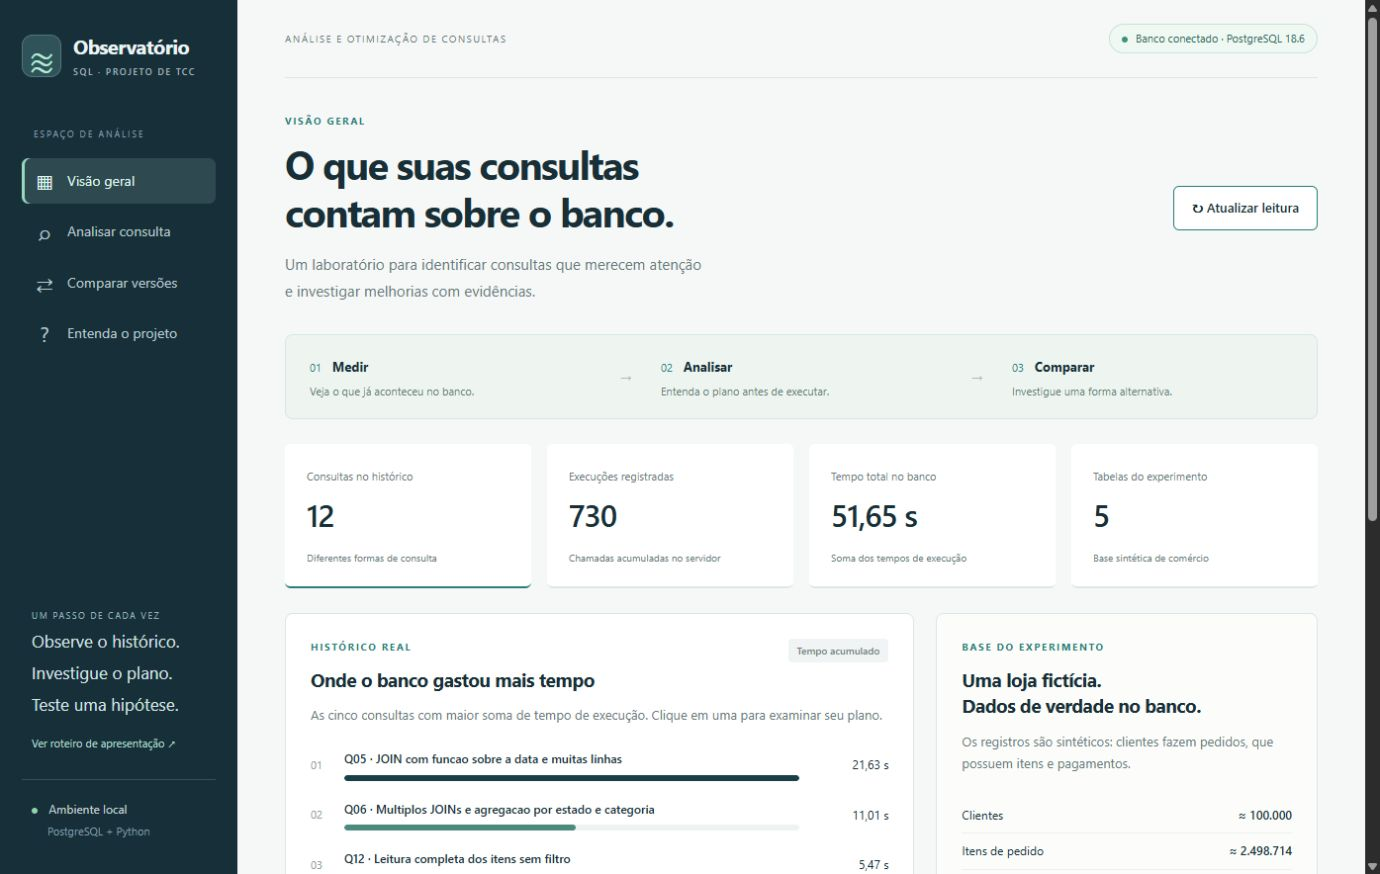
\includegraphics[width=0.88\textwidth]{images/interface.png}
\fonteautor
\end{figure}

Na tela de análise, o usuário pode escolher um exemplo ou colar uma instrução \texttt{SELECT}. O sistema mostra o plano estimado, os sinais encontrados e uma explicação de cada sugestão. Na tela de comparação, a versão original e a alternativa são apresentadas lado a lado. Essa organização permite demonstrar o funcionamento do projeto sem depender apenas do terminal.

Uma verificação posterior confirmou a carga com 730 chamadas e a leitura das 12 consultas pela interface. Também foram testados a rejeição de SQL inválido, o caso de uma consulta sem histórico e a análise sem execução da consulta candidata. Esses testes verificaram o funcionamento do protótipo, mas não correspondem a uma avaliação de usabilidade com participantes.

\subsection{Limitações dos resultados}

O estudo utilizou dados fictícios, valores de filtro fixos e quantidades de chamadas definidas para o experimento. Por isso, os resultados não permitem afirmar que a mesma classificação ocorreria em uma empresa real. Além disso, os tempos podem variar conforme o computador, o uso de memória e outros programas em execução.

A Q12 teve somente uma chamada e, portanto, seu tempo não representa várias observações. A consulta por ano teve apenas uma comparação preventiva de planos. Já o ganho da busca por e-mail depende de os endereços estarem armazenados em letras minúsculas. Essas condições precisam ser mencionadas ao apresentar os resultados.

O protótipo foi desenvolvido para PostgreSQL e uso local. Sua aplicação em produção exigiria novos testes, controle de permissões e avaliação com diferentes consultas e volumes de dados.

\section{CONCLUSÃO}

Este trabalho desenvolveu um processo para identificar e analisar consultas SQL com possíveis problemas de desempenho. A solução combinou estatísticas históricas do PostgreSQL, planos de execução, regras de análise e uma interface web.

Os resultados mostraram que tempo total, tempo médio e frequência destacam situações diferentes. A consulta de pedidos por ano apresentou o maior tempo acumulado, a leitura de todos os itens teve a maior duração em uma única chamada e a busca pela chave primária foi a mais frequente. Assim, uma consulta não deve ser escolhida para análise com base em apenas um número.

Na consulta de pedidos por ano, a alteração do filtro aproximou a quantidade prevista da quantidade observada no histórico, mas não foi medida como otimização. Na busca por e-mail, a comparação direta permitiu o uso do índice existente e reduziu o tempo médio do servidor de 26,33 para 0,0303 milissegundo, mantendo o mesmo resultado nas condições avaliadas.

Concluiu-se que a combinação de histórico e planos pode ajudar a localizar consultas relevantes e explicar por que uma alteração merece ser testada. A ferramenta não modifica automaticamente o banco e não substitui a validação. Sua função é organizar as evidências e apoiar a decisão do desenvolvedor.

Como continuidade, podem ser realizados novos testes com diferentes valores de entrada, mais repetições e outros bancos de dados. Também pode ser feita uma avaliação da interface com usuários para verificar se as explicações são suficientemente claras.


% A versão detalhada abaixo permanece somente como registro de revisão e não é compilada.
\iffalse
\section{MATERIAIS E MÉTODOS}

Iniciou-se a parte prática da pesquisa com a construção de um protótipo para executar consultas SQL, coletar suas estatísticas, analisar seus planos de execução e organizar os resultados obtidos. A pesquisa foi realizada em um ambiente controlado, utilizando dados fictícios e consultas preparadas especificamente para o experimento.

O desenvolvimento foi dividido em seis etapas. Na primeira etapa, construiu-se o banco de dados experimental e definiu-se a estrutura das tabelas e de seus relacionamentos. O objetivo foi disponibilizar uma base com volume suficiente para produzir diferentes comportamentos durante a execução das consultas.

Na segunda etapa, geraram-se os dados fictícios de clientes, produtos, pedidos, itens de pedido e pagamentos. O objetivo foi criar variações nas datas, nos valores, nas situações dos pedidos e na frequência de compra dos clientes.

Na terceira etapa, executou-se uma carga composta por 12 consultas SQL com diferentes filtros, junções, agrupamentos, ordenações e quantidades de chamadas. Essa execução teve como objetivo produzir um histórico que permitisse comparar o tempo total, o tempo médio e a frequência das consultas.

Na quarta etapa, coletaram-se as estatísticas registradas pelo PostgreSQL. As consultas foram classificadas de acordo com o tempo total de execução, o tempo médio por chamada e a quantidade de chamadas, permitindo selecionar os casos considerados mais relevantes para investigação.

Na quinta etapa, analisaram-se os planos de execução das consultas selecionadas. Foram observados sinais como varreduras sequenciais em tabelas grandes, funções aplicadas em filtros, respostas com grande quantidade de linhas e diferenças entre a quantidade estimada e a quantidade histórica de registros.

Na sexta etapa, compararam-se os planos das consultas originais com possíveis alternativas. Para a busca por e-mail, realizou-se também uma avaliação do resultado retornado e do tempo de execução. A comparação por datas permaneceu preventiva, sem medição do tempo da alternativa. Desenvolveu-se, ainda, uma interface web local para apresentar as consultas, as estatísticas, os planos e os sinais identificados.

A Figura~\ref{fig:fluxo-solucao} apresenta essas seis etapas na mesma ordem adotada no desenvolvimento. A geração do histórico envolveu a execução real das consultas. Já a análise preventiva solicitou apenas o plano estimado; a medição de uma alternativa ocorreu separadamente, na etapa de validação.

\begin{figure}[H]
\centering
\caption{Etapas da solução desenvolvida}
\label{fig:fluxo-solucao}
\begin{tikzpicture}[
etapa/.style={rectangle,draw=black,rounded corners,align=center,
  text width=10.7cm,minimum height=0.87cm,font=\small},
seta/.style={-{Latex[length=2mm]},thick},node distance=0.42cm]
\node[etapa] (e1) {1. Construção do banco experimental\\Definição das tabelas, restrições e relacionamentos};
\node[etapa,below=of e1] (e2) {2. Geração e carregamento dos dados fictícios\\Criação de volume e distribuições controladas};
\node[etapa,below=of e2] (e3) {3. Execução da carga de consultas\\Produção do histórico de chamadas, tempos e linhas};
\node[etapa,below=of e3] (e4) {4. Coleta e classificação das estatísticas\\Seleção de casos relevantes para investigação};
\node[etapa,below=of e4] (e5) {5. Análise preventiva dos planos\\Identificação de sinais de atenção e comparação de hipóteses};
\node[etapa,below=of e5] (e6) {6. Validação de uma alteração selecionada\\Comparação dos resultados e medição dos tempos};
\draw[seta] (e1) -- (e2);
\draw[seta] (e2) -- (e3);
\draw[seta] (e3) -- (e4);
\draw[seta] (e4) -- (e5);
\draw[seta] (e5) -- (e6);
\end{tikzpicture}
\fonteautor
\end{figure}

\subsection{Ambiente de desenvolvimento}

O ambiente da primeira rodada experimental utilizou PostgreSQL 18.1 em Windows de 64 bits, Python 3.14.3 e a biblioteca Psycopg 3.3.6 para comunicação entre os programas e o banco de dados. O PostgreSQL foi responsável por armazenar os registros, executar as consultas e produzir os planos. O Python foi utilizado para gerar os dados, organizar as execuções, consultar as métricas e apresentar os resultados. O Psycopg realizou a conexão entre esses componentes.

O DBeaver foi utilizado para administrar a base e conferir as informações. Por meio dessa ferramenta, foi possível inspecionar tabelas, executar os scripts SQL e consultar as quantidades de registros. Também foi criado um ambiente virtual Python para separar as dependências do projeto das demais instalações do computador. Essa separação permitiu registrar as bibliotecas utilizadas e preparar novamente o ambiente quando necessário.

Após a reinstalação do computador, realizou-se uma verificação adicional com PostgreSQL 18.6, Python 3.14.7 e a mesma versão 3.3.6 do Psycopg. A configuração física verificada durante a revisão foi composta por processador AMD Ryzen 5 5600X, com seis núcleos e 12 processadores lógicos, aproximadamente 32~GB de memória RAM, SSD Kingston NV2 de 2~TB e Windows 11 Pro. Essa descrição caracteriza o ambiente local disponível na revisão. Não houve registro detalhado do hardware e dos processos concorrentes no momento da primeira rodada, o que limita sua reprodução exata.

As medições da instalação original foram mantidas separadas das verificações posteriores. Essa distinção foi necessária porque versões do software, estado do cache, estatísticas do banco e atividade de outros programas podem influenciar os tempos. Assim, uma diferença entre rodadas não foi interpretada automaticamente como efeito de otimização.

Os arquivos foram organizados em pastas para scripts SQL, programas Python, documentação, testes, interface e resultados. Os scripts SQL definiram a estrutura da base e as consultas. Os programas Python implementaram geração, carga, coleta e análise. A documentação registrou os procedimentos e as medições disponíveis, enquanto os resultados foram armazenados em arquivos próprios para cada rodada.

As configurações de conexão foram mantidas fora do código, em arquivo de ambiente. Definiram-se regras de versionamento para não incluir credenciais locais no Git. A interface foi disponibilizada apenas no endereço local \texttt{127.0.0.1}, na porta 8765, utilizando o mesmo banco experimental. Não houve implantação em servidor de produção nem avaliação com acesso simultâneo de usuários.

\subsection{Banco experimental e geração dos dados}

Foi criado o banco \texttt{tcc\_sql\_optimizer}, com uma estrutura baseada em operações de um sistema comercial. O modelo contém cinco tabelas: clientes, produtos, pedidos, itens de pedido e pagamentos. Esses relacionamentos permitem identificar o cliente de cada pedido, os produtos comprados e os pagamentos associados.

A tabela de clientes contém identificador, nome, e-mail, cidade, estado, data de cadastro e indicação de situação ativa. O identificador foi definido como chave primária, e o e-mail recebeu uma restrição de unicidade. Essa restrição evita e-mails repetidos e fornece um índice que pôde ser utilizado no experimento de busca por e-mail. A tabela de produtos contém identificador, nome, categoria, preço, estoque e situação ativa.

A tabela de pedidos reúne o cliente responsável, a data, a situação e o valor total de cada compra. Sua relação com clientes foi implementada por uma chave estrangeira. A tabela de itens de pedido associa um pedido a um produto e registra quantidade e valor unitário. Dessa forma, um pedido pode conter vários itens, e um produto pode aparecer em diferentes pedidos. A tabela de pagamentos referencia o pedido e armazena data, forma, valor e situação do pagamento.

\begin{table}[H]
\centering
\caption{Tabelas e relacionamentos da base experimental}
\label{tab:modelo}
\begin{singlespace}\small
\begin{tabularx}{\linewidth}{p{2.4cm} Y Y}
\toprule
\textbf{Tabela} & \textbf{Informação principal} & \textbf{Relacionamento}\\
\midrule
Clientes & Dados de cadastro e identificação. & Um cliente pode possuir vários pedidos.\\[0.5em]
Produtos & Catálogo, preço, estoque e categoria. & Um produto pode aparecer em vários itens de pedido.\\[0.5em]
Pedidos & Data, situação e valor de uma compra. & Cada pedido referencia um cliente.\\[0.5em]
Itens de pedido & Produto, quantidade e valor unitário. & Cada item referencia um pedido e um produto.\\[0.5em]
Pagamentos & Forma, situação, data e valor pago. & Cada pagamento referencia um pedido.\\
\bottomrule
\end{tabularx}
\fonteautor
\end{singlespace}
\end{table}

Todas as tabelas receberam chaves primárias. As chaves estrangeiras impediram referências a clientes, produtos e pedidos inexistentes. Outras restrições limitaram preços e estoques a valores não negativos, quantidades de itens a valores positivos e situações de pedidos e pagamentos aos conjuntos definidos. No conjunto gerado, produziu-se um pagamento por pedido; essa proporção foi uma regra do gerador, não uma restrição de unicidade da coluna que referencia o pedido.

O esquema inicial criou os índices decorrentes das chaves primárias e da unicidade do e-mail. Não foram acrescentados índices específicos nas datas, nas chaves estrangeiras ou na expressão \texttt{LOWER(email)}. Essa configuração permitiu observar tanto buscas por índices já existentes quanto consultas que precisavam percorrer grandes tabelas. A ausência desses índices adicionais foi uma condição do cenário experimental, e não uma recomendação para sistemas comerciais.

A base foi preenchida com dados fictícios por meio de um programa em Python desenvolvido com auxílio de inteligência artificial. O programa gerou os registros automaticamente, e o carregamento foi realizado em lotes de 10.000 linhas, utilizando o mecanismo \texttt{COPY} do PostgreSQL, destinado à transferência de dados entre tabelas e fontes de entrada ou saída \cite{postgresql2026copy}. O programa verificou se as tabelas estavam vazias antes da carga, confirmou a transação ao final e executou \texttt{ANALYZE} nas cinco tabelas para atualizar as estatísticas utilizadas pelo planejador.

Ao final, foram conferidos 100.000 clientes, 50.000 produtos, 1.000.000 de pedidos, 2.498.714 itens de pedido e 1.000.000 de pagamentos, totalizando 4.648.714 registros. A Tabela~\ref{tab:volumes} apresenta as quantidades e sua função no experimento.

\begin{table}[H]
\centering
\caption{Volumes utilizados e sua justificativa experimental}
\label{tab:volumes}
\begin{singlespace}\small
\begin{tabularx}{\linewidth}{p{2.5cm} r Y}
\toprule
\textbf{Tabela} & \textbf{Registros} & \textbf{Justificativa}\\
\midrule
Clientes & 100.000 & Permitir buscas seletivas por identificador e e-mail e distribuição desigual dos pedidos.\\[0.5em]
Produtos & 50.000 & Compor um catálogo com categorias, preços e diferentes frequências de compra.\\[0.5em]
Pedidos & 1.000.000 & Produzir volume para filtros temporais, junções, agrupamentos e ordenações.\\[0.5em]
Itens de pedido & 2.498.714 & Ampliar as junções e permitir uma consulta que devolve milhões de linhas.\\[0.5em]
Pagamentos & 1.000.000 & Manter um pagamento por pedido na geração e permitir filtros por situação e forma.\\
\midrule
\textbf{Total} & \textbf{4.648.714} & Conjunto com diferentes escalas de leitura e retorno.\\
\bottomrule
\end{tabularx}
\fonteautor
\end{singlespace}
\end{table}

As quantidades foram decisões de dimensionamento do experimento. Buscou-se um contraste entre acessos a uma linha e operações sobre centenas de milhares ou milhões de registros, mantendo a carga executável no computador local. O milhão de pedidos corresponde, em média, a dez pedidos por cliente, mas a distribuição foi deliberadamente desigual. Os dois ou três itens de cada pedido produziram uma tabela maior, útil para observar o impacto de respostas extensas. Esses volumes não foram derivados de uma empresa real, de uma amostragem estatística ou de um padrão de teste de desempenho.

A geração incluiu variações na frequência de compra dos clientes, na procura pelos produtos, nos preços e nas datas e situações dos pedidos. Para permitir a repetição do processo, foi definido um valor fixo de inicialização da geração pseudoaleatória, chamado de semente. O valor escolhido foi 2026. Mantidos o programa e seus parâmetros, a semente reproduz a sequência de escolhas; ela não garante tempos de execução idênticos, pois estes também dependem do ambiente.

Oitenta por cento dos sorteios de cliente para um pedido foram concentrados nos primeiros 20\% dos clientes. De forma semelhante, 70\% dos sorteios de produto foram concentrados nos primeiros 10\% do catálogo. Essas escolhas criaram grupos com maior atividade, permitindo observar filtros que atingem parcelas diferentes da base. As datas de pedidos foram distribuídas entre 2024, 2025 e 2026 com pesos de 20\%, 30\% e 50\%, respectivamente; no último ano, o intervalo gerado terminou antes de 1º de setembro.

Os pedidos receberam as situações pendente, pago, enviado, entregue ou cancelado, com pesos de 12\%, 13\%, 20\%, 48\% e 7\%. Cada pedido recebeu dois ou três itens, e seu valor total foi calculado a partir das quantidades e dos valores unitários. A situação do pagamento foi relacionada à situação do pedido. Os e-mails foram gerados em letras minúsculas, condição relevante para a validade da reescrita avaliada posteriormente.

Para verificar a consistência, prepararam-se consultas que identificaram pedidos com quantidade inválida de itens, divergências entre soma dos itens e total do pedido, pagamentos ausentes ou de valor incompatível, datas incoerentes e situações incompatíveis. Também foram verificadas as contagens das tabelas e a concentração de pedidos no grupo de clientes frequentes. A base foi tratada como cenário experimental, sem afirmar que sua distribuição representa o comportamento de uma empresa real.

\subsection{Consultas e execução da carga}

Foram elaboradas 12 consultas SQL envolvendo filtros, junções entre tabelas, agrupamentos, ordenações, cálculos e subconsultas. O conjunto inclui buscas que retornam poucos registros e operações que retornam grandes volumes de dados. Também foram incluídas construções potencialmente custosas para investigação posterior à coleta, preservando-se as formas originais durante a carga de referência.

As consultas receberam identificadores locais de Q01 a Q12, usados apenas para organização do experimento. Esses nomes não são os identificadores internos calculados pelo PostgreSQL. A Tabela~\ref{tab:consultas} apresenta o perfil de cada consulta antes de sua discussão nos resultados.

\begin{table}[H]
\centering
\caption{Consultas e frequências definidas para a carga}
\label{tab:consultas}
\begin{singlespace}\small
\begin{tabularx}{\linewidth}{c r Y}
\toprule
\textbf{Consulta} & \textbf{Chamadas} & \textbf{Operação principal}\\
\midrule
Q01 & 500 & Busca de cliente pela chave primária.\\[0.35em]
Q02 & 100 & Filtro de produtos por categoria, preço e situação, com ordenação e limite.\\[0.35em]
Q03 & 60 & Consulta de pedidos de um cliente, ordenados pela data.\\[0.35em]
Q04 & 20 & Seleção de todas as colunas de pedidos cancelados.\\[0.35em]
Q05 & 15 & Junção entre pedidos e clientes com extração do ano da data.\\[0.35em]
Q06 & 10 & Junção das cinco tabelas e agregação por estado e categoria.\\[0.35em]
Q07 & 8 & Agregação mensal de pedidos em um intervalo de datas.\\[0.35em]
Q08 & 6 & Ordenação dos pedidos de maior valor, com limite de 1.000 linhas.\\[0.35em]
Q09 & 5 & Busca de cliente com aplicação de \texttt{LOWER} ao e-mail.\\[0.35em]
Q10 & 3 & Seleção de pedidos acima do valor médio, calculado por subconsulta.\\[0.35em]
Q11 & 2 & Subconsulta correlacionada para contar pedidos de clientes.\\[0.35em]
Q12 & 1 & Leitura de todos os itens de pedido, sem filtro.\\
\midrule
\textbf{Total} & \textbf{730} & Frequências definidas para o cenário experimental.\\
\bottomrule
\end{tabularx}
\fonteautor
\end{singlespace}
\end{table}

Um programa Python foi desenvolvido para executar as consultas com frequências definidas, variando de uma a 500 chamadas por consulta. Essas frequências foram estabelecidas para o experimento e não foram obtidas do uso de um sistema real. A diferença entre elas permitiu comparar uma consulta frequente e seletiva com consultas menos frequentes e mais volumosas.

Inicialmente, foi realizado um teste funcional com uma execução de cada consulta. Em seguida, foi executada a carga completa, composta por 730 chamadas. Nessa rodada, os valores dos filtros foram mantidos fixos. Não houve, portanto, avaliação do comportamento das consultas com diferentes valores de entrada.

O programa preparou uma lista contendo as repetições de cada consulta e embaralhou sua ordem com semente 2026. A sessão de execução foi configurada como somente leitura e com limite de 120 segundos por comando. Os resultados foram consumidos pelo cliente, de modo que a medição no Python incluiu o processamento necessário para recebê-los. Não foi simulado um conjunto de usuários concorrentes.

O registro da primeira rodada informa o horário de coleta, mas não preserva o horário de reinicialização das estatísticas. Por esse motivo, a correspondência entre 730 chamadas previstas e observadas foi utilizada como verificação de contagem, sem ser apresentada como comprovação completa do isolamento da janela. Na verificação posterior do ambiente, documentou-se que o conjunto filtrado estava vazio antes da carga completa.

\subsection{Coleta e classificação das consultas}

A coleta utilizou a extensão \texttt{pg\_stat\_statements}, versão 1.12. A fonte de análise consistiu em estatísticas acumuladas das consultas, e não em arquivos de log com um registro separado para cada execução. Esse recorte delimita o uso de informações históricas neste trabalho. A extensão associa métricas a comandos normalizados; valores literais diferentes podem compartilhar a mesma entrada de histórico \cite{postgresql2026pgstat}.

Foi desenvolvido um coletor em Python para consultar essas informações e selecionar os comandos relacionados às tabelas experimentais. Aplicaram-se filtros de banco, usuário e consulta para reduzir a presença de comandos administrativos e de outras operações fora do conjunto analisado. A identificação local de Q01 a Q12 foi associada ao conteúdo SQL, enquanto o identificador interno do PostgreSQL foi preservado nos registros exportados.

As consultas foram organizadas em três classificações: tempo total de execução, tempo médio por execução e quantidade de chamadas. O tempo total foi utilizado para observar a duração acumulada; o tempo médio, para comparar a duração por chamada; e a frequência, para identificar as consultas mais executadas. Também se registrou a quantidade acumulada de linhas retornadas, relevante para interpretar consultas com respostas muito diferentes.

O cálculo da média histórica de linhas por chamada foi definido pela divisão do total de linhas pelo número de chamadas. Essa média foi utilizada como referência para comparação com a saída estimada do plano. Como o histórico é agregado, essa relação não representa necessariamente um parâmetro específico quando os valores de entrada variam. No experimento principal, os filtros foram mantidos fixos, reduzindo essa ambiguidade.

A implementação também incluiu um indicador calculado pela multiplicação do tempo médio pela quantidade de chamadas. Como esse cálculo reproduz aproximadamente o tempo total, ele não foi tratado como uma medida independente na análise apresentada. Sua presença na implementação não alterou os três critérios de classificação adotados no estudo.

O tempo registrado pelo programa Python foi mantido separado dos tempos coletados no PostgreSQL. O primeiro corresponde à duração medida pelo programa para executar a carga, enquanto os demais são as métricas de execução fornecidas pelo banco. Esses valores não foram considerados equivalentes, pois a medição no cliente também abrange comunicação, conversão e tratamento dos resultados.

Foi implementada a exportação das métricas para CSV e JSON. O CSV organizou os registros em colunas para conferência tabular; o JSON preservou os dados estruturados e os metadados de coleta. Os resultados da primeira rodada foram documentados a partir das saídas de terminal, com valores arredondados. Na verificação posterior, os arquivos exportados foram conferidos campo a campo. Essa distinção mantém explícita a origem das evidências disponíveis em cada momento.

\subsection{Análise preventiva dos planos de execução}

Implementou-se a análise preventiva para examinar uma consulta antes de executá-la para medição. O programa recebeu um único comando \texttt{SELECT}, solicitou seu plano ao PostgreSQL e organizou as informações em formato JSON. A solicitação utilizou \texttt{EXPLAIN} com \texttt{ANALYZE FALSE}, preservando a distinção entre planejamento e execução. O custo fornecido pelo planejador foi interpretado como unidade de comparação de planos, não como duração em milissegundos \cite{postgresql2026explain}.

A entrada foi restringida a uma única instrução de consulta. Comandos de alteração, múltiplas instruções, \texttt{SELECT INTO} e construções com \texttt{WITH} foram rejeitados pelo validador implementado. Além dessa restrição, a conexão foi configurada como somente leitura e foram utilizados limites de tempo. Essas medidas definiram o escopo do protótipo; não constituem uma prova de segurança para qualquer expressão SQL possível.

O plano foi percorrido como uma árvore de operações. Foram identificados o nó principal, as relações acessadas, os filtros, as quantidades estimadas de linhas e os custos. Um nó do tipo \texttt{Seq Scan} indica leitura sequencial; \texttt{Index Scan} indica uso de índice; e nós de junção, ordenação e subconsulta descrevem outras partes do processamento. A análise considerou cada operação em seu contexto, evitando classificar todo acesso sequencial como falha.

Definiram-se regras heurísticas, isto é, critérios práticos para destacar situações que merecem investigação. Os limiares foram escolhas do protótipo e não foram obtidos de um treinamento estatístico. A Tabela~\ref{tab:regras} apresenta os sinais e os pontos atribuídos. Ocorrências idênticas foram removidas antes da soma; o escore final foi limitado a dez.

\begin{table}[H]
\centering
\caption{Regras utilizadas para atribuição do nível de atenção}
\label{tab:regras}
\begin{singlespace}\small
\begin{tabularx}{\linewidth}{Y p{7.0cm} c}
\toprule
\textbf{Sinal} & \textbf{Condição observada} & \textbf{Pontos}\\
\midrule
Seleção ampla & Presença de \texttt{SELECT *}. & 1\\[0.5em]
Varredura sequencial & Filtro em relação com pelo menos 50.000 linhas estimadas. & 3\\[0.5em]
Função no filtro & Expressões reconhecidas, como \texttt{EXTRACT} e \texttt{LOWER}. & 2\\[0.5em]
Ordenação extensa & Nó de ordenação com pelo menos 10.000 linhas estimadas. & 2\\[0.5em]
Laço aninhado & Produto das linhas estimadas dos dois primeiros ramos de pelo menos 1.000.000. & 2\\[0.5em]
Resultado volumoso & Saída estimada de pelo menos 100.000 linhas. & 3\\[0.5em]
Divergência de linhas & Razão de pelo menos dez entre a maior e a menor quantidade estimada e histórica, para valores positivos. & 3\\[0.5em]
Subplano & Presença de operação identificada como subplano. & 2\\
\bottomrule
\end{tabularx}
\fonteautor
\end{singlespace}
\end{table}

Escores de zero a dois foram classificados como atenção baixa; de três a seis, como média; e de sete a dez, como alta. O escore não representa probabilidade de falha, tempo esperado ou percentual de melhoria. Sua função é organizar os sinais encontrados e ajudar a selecionar o que deve ser investigado.

Para cada sinal, o sistema apresentou uma evidência e uma sugestão. No caso de função aplicada ao filtro de data, a sugestão foi avaliar uma comparação por intervalo. Para uma varredura em tabela grande, recomendou-se verificar a seletividade e os índices disponíveis. Nenhuma regra criou índices ou modificou consultas automaticamente. O resultado foi apresentado como hipótese dependente de avaliação posterior.

\subsection{Comparação de alternativas e validação}

Selecionaram-se dois casos para comparação: a consulta de pedidos por ano e a busca de cliente por e-mail. A primeira reuniu elevado tempo acumulado e uma função aplicada à data. A segunda permitiu examinar o efeito de aplicar uma função a uma coluna que já possuía índice de unicidade. A escolha combinou impacto histórico e possibilidade de explicar uma mudança concreta no plano.

Na comparação preventiva, solicitou-se o plano da consulta original e o da alternativa. Compararam-se método de acesso, custo, linhas estimadas e sinais de atenção. A consulta por ano foi reescrita com limites de data. A busca por e-mail foi reescrita como comparação direta. Essas alternativas foram preparadas para o experimento; o protótipo não gerou automaticamente uma nova instrução SQL.

Para medir o desempenho, selecionou-se a busca por e-mail. A condição conhecida da geração, em que todos os e-mails foram armazenados em minúsculas, fundamentou a comparação direta. Utilizou-se o mesmo valor de busca nas duas formas. O programa comparou os primeiros conjuntos de resultados retornados e contabilizou as linhas das chamadas seguintes. Não foi implementada uma prova geral de equivalência entre consultas arbitrárias.

Executaram-se 100 chamadas de cada versão, intercaladas em ordem pseudoaleatória com semente 2026. As estatísticas foram lidas antes e depois da rodada, sem reinicialização do \texttt{pg\_stat\_statements}. Para isolar as 100 chamadas de cada forma, calcularam-se as diferenças entre os contadores finais e iniciais. O tempo médio da rodada foi obtido pela diferença do tempo total dividida pela diferença do número de chamadas.

A redução percentual de tempo foi calculada por:
\begin{equation}
R = \frac{T_{\mathrm{original}}-T_{\mathrm{alternativa}}}{T_{\mathrm{original}}}\times 100,
\label{eq:reducao}
\end{equation}
em que $T_{\mathrm{original}}$ e $T_{\mathrm{alternativa}}$ representam os tempos médios da mesma métrica. Aplicou-se o cálculo separadamente às medidas do servidor e do cliente. Não se misturaram tempos de camadas diferentes na mesma redução percentual.

\subsection{Interface e verificação funcional}

Desenvolveu-se uma interface web local, denominada Observatório SQL, para tornar as informações acessíveis sem exigir a execução manual de cada módulo. A interface utilizou um servidor Python e os mesmos componentes de coleta e análise da linha de comando. Sua finalidade foi apoiar a interpretação e a demonstração do protótipo.

A interface foi organizada em quatro áreas. A visão geral apresentou o histórico e o ranking de consultas. A área de análise permitiu selecionar um exemplo ou informar uma consulta. A comparação apresentou os planos de duas versões. A área didática reuniu explicações sobre plano, custo, índice, linhas estimadas e histórico. Em todas as análises preventivas, informou-se que o \texttt{SELECT} candidato não seria executado para medir tempo.

Prepararam-se testes automatizados das respostas HTTP e verificações de integração com o banco. Foram examinados o funcionamento de uma consulta sem histórico, a rejeição de entradas inválidas e a preservação dos contadores das consultas do experimento ao usar as funções preventivas. Esses testes verificaram o funcionamento do protótipo; não substituíram a avaliação de desempenho das consultas.


\section{RESULTADOS E DISCUSSÃO}

Os resultados apresentados incluem a primeira rodada de execução e coleta, as análises preventivas e a validação de uma reescrita. As verificações realizadas após a reinstalação do ambiente são identificadas separadamente. Essa organização preserva os resultados da rodada original e evita comparar tempos obtidos em momentos diferentes como se pertencessem ao mesmo experimento.

\subsection{Execução e coleta das métricas}

O teste funcional executou as 12 consultas sem erros, com duração aproximada de 14,3 segundos no programa Python. A carga completa também foi concluída sem erros, totalizando 730 execuções em aproximadamente 103,2 segundos, conforme a medição do programa.

Na coleta apresentada, foram selecionadas 12 consultas, com um total de 730 chamadas. Outras 13 entradas foram excluídas pelo filtro do coletor. Essa correspondência constituiu uma verificação de contagem do conjunto analisado. O registro da coleta informa 29 de setembro de 2026, às 17:48:14 UTC. Como o horário de reinicialização das estatísticas não foi registrado, permaneceu uma limitação na documentação da janela da primeira rodada.

Os números dessa rodada foram preservados no registro do experimento a partir dos valores exibidos no terminal. Os valores arredondados não permitem recuperar toda a precisão interna do PostgreSQL. Ainda assim, permitem comparar os critérios de classificação e identificar os casos posteriormente investigados, desde que sua origem seja explicitada.

\subsection{Comparação dos critérios de classificação}

A consulta Q05, que relaciona pedidos e clientes e utiliza \texttt{EXTRACT} no filtro de ano, apresentou o maior tempo total: aproximadamente 42,47 segundos em 15 chamadas. Seu tempo médio foi de 2,83 segundos. Esse resultado a tornou um caso prioritário para investigação dentro da carga executada. O ranking, isoladamente, não permite atribuir esse tempo ao filtro, à junção ou a uma operação específica; os sinais do plano são discutidos na subseção seguinte.

A consulta Q12, que realiza a leitura de todos os itens de pedido, apresentou o maior tempo médio, de aproximadamente 6,80 segundos. Como foi executada uma única vez, esse valor corresponde a uma observação isolada. Além disso, a consulta retornou 2.498.714 linhas, característica que deve ser considerada na comparação com buscas que produzem respostas menores.

A consulta Q01, que busca um cliente pela chave primária, foi a mais frequente, com 500 chamadas. Apesar disso, seu tempo total registrado no servidor foi de aproximadamente 9,25 milissegundos. O caso mostra que uma frequência elevada, por si só, não implica maior tempo acumulado.

\begin{table}[H]
\centering
\caption{Consultas destacadas pelos critérios de classificação}
\label{tab:rankings}
\begin{singlespace}\small
\begin{tabularx}{\linewidth}{c r r r Y}
\toprule
\textbf{Consulta} & \textbf{Chamadas} & \textbf{Total (ms)} & \textbf{Média (ms)} & \textbf{Destaque}\\
\midrule
Q05 & 15 & 42.472,08 & 2.831,47 & Maior tempo acumulado.\\[0.5em]
Q12 & 1 & 6.795,63 & 6.795,63 & Maior duração por chamada.\\[0.5em]
Q01 & 500 & 9,25 & 0,02 & Maior frequência.\\
\bottomrule
\end{tabularx}
\fonteautor
\end{singlespace}
\end{table}

Os critérios destacaram, portanto, consultas diferentes. Q05 concentrou o maior tempo acumulado, Q12 apresentou a maior duração por chamada e Q01 teve o maior número de execuções. Essa diferença justifica observar as três medidas em conjunto ao selecionar os casos de análise. A duração de uma resposta com milhões de registros também deve ser interpretada considerando a necessidade de retornar esse volume ao consumidor.

\subsection{Análise da consulta de pedidos por ano}

A consulta Q05 selecionou pedidos de 2026 e os dados dos clientes relacionados. A condição original extraiu o ano de cada data. Sua estrutura foi:

\begin{lstlisting}[language=SQL]
SELECT *
FROM public.pedidos p
JOIN public.clientes c ON c.id = p.cliente_id
WHERE EXTRACT(YEAR FROM p.data_pedido) = 2026;
\end{lstlisting}

O plano estimado apresentou cinco nós, operação principal \texttt{Gather}, custo total de 19.003 e estimativa de 5.000 linhas de saída. O histórico registrou 7.495.140 linhas em 15 chamadas, equivalentes a uma média de 499.676 linhas por execução. A quantidade histórica foi aproximadamente 99,9 vezes maior que a estimativa.

Na versão do analisador que incluiu a regra de divergência de cardinalidade, foram encontrados quatro sinais: seleção de todas as colunas, varredura sequencial com filtro na tabela de pedidos, função aplicada à data e diferença elevada entre a quantidade estimada e a histórica. A soma resultou em atenção alta, com escore 9/10. Esse valor sintetizou os sinais encontrados, sem representar uma previsão de duração.

A alternativa substituiu a extração do ano por um intervalo fechado no início e aberto no fim. Mantiveram-se a seleção e a junção:

\begin{lstlisting}[language=SQL]
WHERE p.data_pedido >= TIMESTAMP '2026-01-01 00:00:00'
  AND p.data_pedido <  TIMESTAMP '2027-01-01 00:00:00';
\end{lstlisting}

Na comparação registrada, a alternativa apresentou quatro nós, operação principal \texttt{Hash Join} e estimativa de 499.434 linhas. A diferença em relação à média histórica foi de 242 linhas, aproximadamente 0,05\%. O alerta de função aplicada ao filtro desapareceu. O escore permaneceu alto, em 7/10, devido aos demais sinais, incluindo o grande volume de saída.

\begin{table}[H]
\centering
\caption{Comparação preventiva do filtro de ano e do intervalo de datas}
\label{tab:datas}
\begin{singlespace}\small
\begin{tabularx}{\linewidth}{Y r r}
\toprule
\textbf{Métrica} & \textbf{Filtro com função} & \textbf{Intervalo de datas}\\
\midrule
Operação principal & Gather & Hash Join\\[0.4em]
Nós no plano & 5 & 4\\[0.4em]
Custo estimado & 19.003,00 & 38.633,07\\[0.4em]
Linhas estimadas & 5.000 & 499.434\\[0.4em]
Nível de atenção & Alto, 9/10 & Alto, 7/10\\
\bottomrule
\end{tabularx}
\fonteautor
\end{singlespace}
\end{table}

O custo estimado aumentou mesmo com a aproximação da cardinalidade ao histórico. Esse resultado não comprova que a alternativa ficou mais lenta, pois custo não é tempo e os planos passaram a considerar quantidades de linhas muito diferentes. Também não comprova aceleração: nenhuma das duas consultas foi executada durante essa comparação preventiva.

A permanência de varredura sequencial é compatível com uma consulta que seleciona aproximadamente metade da tabela de pedidos. Nessa condição, a existência de um índice não garante benefício. O caso mostrou a utilidade de explicar os sinais em conjunto e de evitar uma recomendação automática baseada apenas na presença de uma operação do plano.

\subsection{Comparação e validação da busca por e-mail}

A consulta Q09 buscou um cliente aplicando \texttt{LOWER} à coluna de e-mail. A função converte letras para minúsculas antes da comparação. No conjunto sintético, entretanto, os valores já estavam armazenados em minúsculas. A comparação preventiva examinou as duas condições abaixo, com a mesma seleção de colunas e o mesmo valor de busca:

\begin{lstlisting}[language=SQL]
-- Condicao original
WHERE LOWER(email) = 'cliente123@example.com';

-- Alternativa avaliada
WHERE email = 'cliente123@example.com';
\end{lstlisting}

O plano original apresentou \texttt{Seq Scan}, custo estimado de 2.868 e previsão de 500 linhas. A alternativa utilizou \texttt{Index Scan}, custo 8,44 e estimativa de uma linha. O índice único da coluna de e-mail já existia; não foi criado um novo índice para produzir esse resultado. A comparação direta permitiu ao planejador utilizar a coluna indexada sem aplicar a função a cada valor.

\begin{table}[H]
\centering
\caption{Planos estimados para a busca por e-mail}
\label{tab:email-planos}
\begin{singlespace}\small
\begin{tabularx}{\linewidth}{Y r r}
\toprule
\textbf{Métrica} & \textbf{Com LOWER} & \textbf{Comparação direta}\\
\midrule
Método de acesso & Seq Scan & Index Scan\\[0.4em]
Custo estimado & 2.868,00 & 8,44\\[0.4em]
Linhas estimadas & 500 & 1\\[0.4em]
Nível de atenção & Alto, 8/10 & Baixo, 0/10\\
\bottomrule
\end{tabularx}
\fonteautor
\end{singlespace}
\end{table}

O histórico da consulta original indicava uma linha por chamada. A estimativa da alternativa coincidiu com essa referência, enquanto a original superestimou o resultado em 500 vezes. O custo estimado diminuiu 99,71\%, mas esse percentual foi tratado somente como resultado do planejamento. A comprovação de redução de tempo dependeu da rodada executada posteriormente.

Na validação real, os primeiros conjuntos de resultados comparados foram iguais. Cada versão retornou uma linha por chamada, totalizando 100 linhas em 100 execuções. A Tabela~\ref{tab:email-tempos} apresenta os tempos acumulados e médios obtidos pelos deltas da rodada.

\begin{table}[H]
\centering
\caption{Medições da validação da busca por e-mail}
\label{tab:email-tempos}
\begin{singlespace}\small
\begin{tabularx}{\linewidth}{Y r r}
\toprule
\textbf{Métrica} & \textbf{Com LOWER} & \textbf{Comparação direta}\\
\midrule
Chamadas & 100 & 100\\[0.4em]
Linhas acumuladas & 100 & 100\\[0.4em]
Tempo total no servidor (ms) & 2.633,00 & 3,03\\[0.4em]
Tempo médio no servidor (ms) & 26,3300 & 0,0303\\[0.4em]
Tempo total no cliente (ms) & 2.671,49 & 39,64\\[0.4em]
Tempo médio no cliente (ms) & 26,7149 & 0,3964\\
\bottomrule
\end{tabularx}
\fonteautor
\end{singlespace}
\end{table}

A redução do tempo médio no servidor foi de aproximadamente 99,88\%. No cliente Python, a redução foi de 98,52\%. A diferença é coerente com a presença de custos de comunicação, biblioteca e processamento do resultado na medição do cliente. Esses custos passam a representar uma parcela maior quando o tempo de execução no servidor se torna muito pequeno.

O resultado confirmou a direção da hipótese preventiva neste conjunto de dados. A condição de equivalência, porém, depende da normalização dos e-mails. Se uma aplicação armazenar letras maiúsculas e minúsculas e exigir uma comparação que ignore essa diferença, retirar \texttt{LOWER} pode alterar a resposta. Por isso, o ganho observado não autoriza a aplicação da mesma reescrita em qualquer banco.

\subsection{Verificações posteriores e apresentação visual}

Após a reinstalação do ambiente, a verificação de 12 de outubro de 2026 confirmou novamente as cinco contagens de tabelas, totalizando 4.648.714 registros. Os cinco indicadores de inconsistência retornaram zero. A concentração observada nos clientes frequentes foi de 80,02\% dos pedidos, compatível com o peso definido no gerador. Essas verificações complementaram a documentação da base, sem alterar retroativamente as condições da rodada inicial.

Nessa verificação posterior, a carga completa registrou 730 chamadas em aproximadamente 55,8 segundos no cliente. O coletor selecionou 12 consultas, e os arquivos CSV e JSON foram conferidos campo a campo. O tempo diferente dos 103,2 segundos da primeira rodada não foi tratado como resultado de otimização, pois se refere a outra execução e a uma instalação diferente.

A interface reuniu histórico, análise preventiva, comparação e explicações em uma apresentação visual. A Figura~\ref{fig:interface} mostra a visão geral registrada na verificação de 13 de outubro de 2026. Os valores exibidos pertencem àquela rodada e não substituem as métricas históricas apresentadas nas subseções anteriores.

\begin{figure}[H]
\centering
\caption{Visão geral da interface web na verificação posterior}
\label{fig:interface}
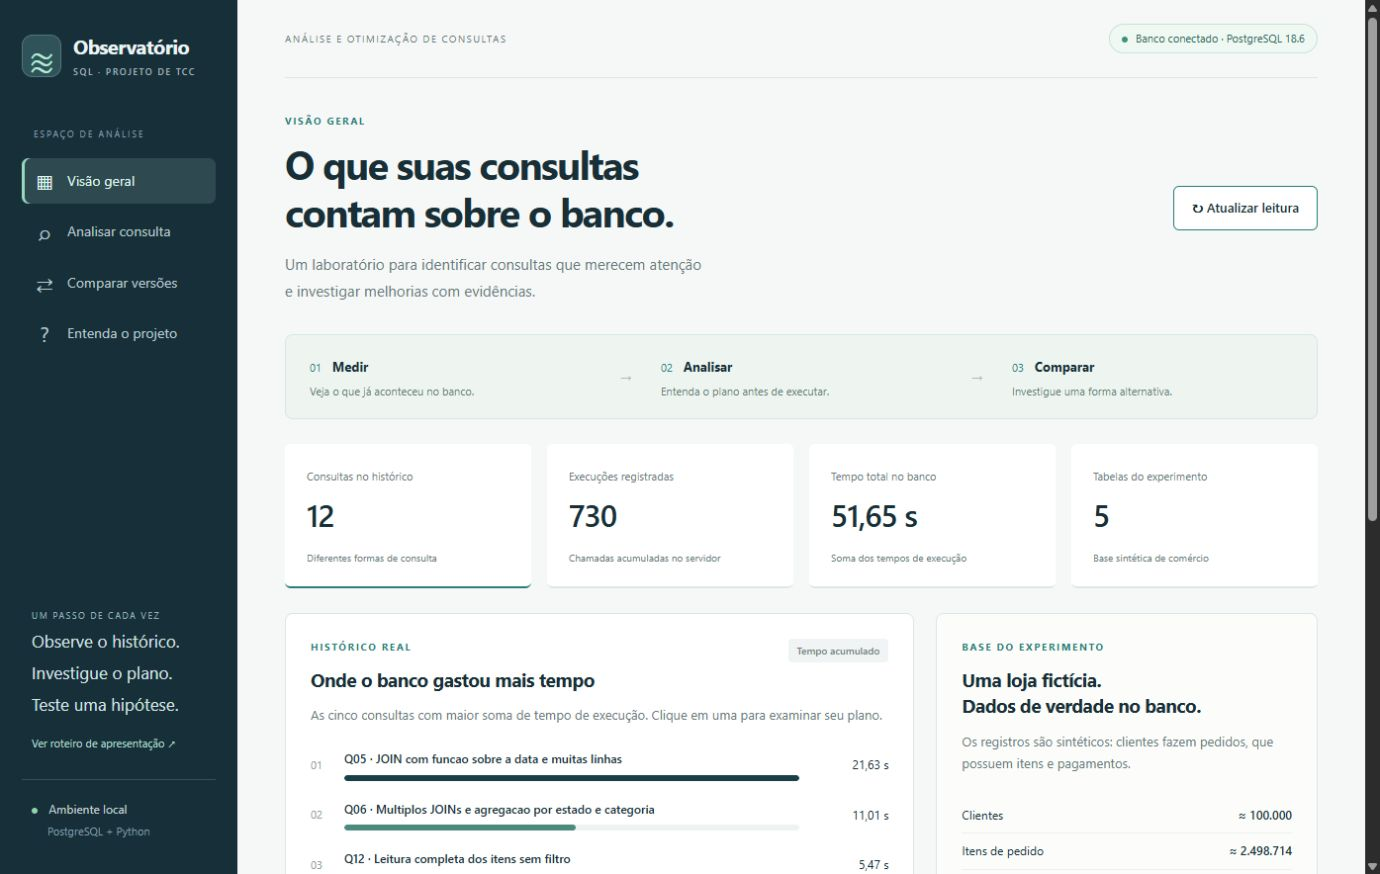
\includegraphics[width=\linewidth]{images/interface.png}
\fonteautor
\end{figure}

Na integração de 13 de outubro, as estatísticas das consultas do experimento permaneceram iguais antes e depois das análises e comparações, com 730 chamadas. Esse resultado foi compatível com o uso de planos estimados sem execução dos comandos candidatos. Também foram verificadas a rejeição de SQL inválido e a análise de uma consulta sem histórico, situação em que o sistema apresentou o plano sem inventar uma duração real.

O registro de verificação apontou sete testes automatizados aprovados para o contrato HTTP. A comparação por e-mail voltou a apresentar acesso sequencial na forma original e uso de índice na alternativa. Esses resultados demonstraram funcionamento das principais operações da interface, mas não constituíram uma avaliação de usabilidade com participantes nem um teste de produção.

\subsection{Limitações dos resultados}

A rodada utilizou dados fictícios, frequências definidas para o experimento e valores fixos nos filtros. Os resultados descrevem essas condições e não permitem afirmar que a mesma classificação ocorreria em um sistema real. A concentração de clientes e produtos e os pesos de datas foram escolhas do cenário, não observações de uma empresa.

A sequência das consultas pode influenciar as medições, pois dados acessados anteriormente podem permanecer em memória e ser reutilizados. A intercalação das versões de e-mail reduziu a associação entre uma versão e um momento específico da rodada, mas não eliminou os efeitos de cache. Não foram calculados intervalos de confiança nem avaliadas várias rodadas independentes, especialmente no caso de Q12, que teve apenas uma execução na carga inicial.

A documentação da primeira rodada não preservou o horário de reinicialização das estatísticas nem uma descrição detalhada dos processos concorrentes. Os arquivos originais de métricas não estavam disponíveis na revisão; os valores dessa rodada foram mantidos a partir do registro de terminal. Os arquivos conferidos posteriormente pertencem à reinstalação e foram tratados como evidências distintas.

O histórico do \texttt{pg\_stat\_statements} é agregado. Consultas com valores diferentes podem compartilhar uma entrada, e sua média de linhas pode não representar um caso individual. A comparação com a cardinalidade estimada deve, portanto, ser interpretada como sinal de investigação. Além disso, os limiares e pesos heurísticos não foram calibrados em um conjunto externo de consultas, o que impede atribuir ao escore uma precisão estatística de diagnóstico.

A preservação do resultado na busca por e-mail foi apoiada pela regra de normalização e pela comparação inicial dos retornos. O protótipo não provou equivalência geral e não testou diferentes valores de entrada. A alternativa por datas foi examinada apenas de forma preventiva. Assim, a conclusão de ganho medido ficou restrita ao caso de e-mail e às condições registradas.

Por fim, o protótipo foi desenvolvido para PostgreSQL e uso local. Outros SGBDs possuem formatos de plano e métricas diferentes. A aplicação em produção também exigiria uma avaliação específica de permissões, carga concorrente, robustez da validação SQL e impacto da própria coleta. Esses aspectos delimitam o alcance do estudo e indicam possibilidades de continuidade.

\section{Conclusão}

Este trabalho teve como objetivo desenvolver e avaliar um processo de análise preventiva de consultas SQL baseado em estatísticas históricas e planos de execução. A combinação dessas informações permitiu identificar consultas relevantes para investigação, explicar os sinais encontrados e comparar possíveis alterações em sua escrita.

A primeira rodada mostrou que tempo total, tempo médio e frequência destacam situações diferentes. A consulta de pedidos por ano concentrou o maior tempo acumulado, a leitura completa dos itens apresentou a maior duração por chamada e a busca pela chave primária foi a mais frequente. Esses resultados reforçaram a necessidade de considerar o volume retornado e o contexto de uso, além de uma única métrica.

Na análise da consulta de pedidos por ano, a comparação por intervalo de datas aproximou a quantidade estimada de linhas da referência histórica. Esse resultado não comprovou ganho de tempo, pois a alternativa não foi executada para medição. Na busca por e-mail, a comparação direta permitiu o uso do índice existente e a validação registrou redução de 99,88\% no tempo médio do servidor. Os primeiros resultados comparados foram iguais, e a validade da alteração ficou condicionada à normalização dos e-mails utilizada na base.

Concluiu-se que a integração de estatísticas, planos e regras explicáveis pode apoiar a identificação de gargalos e a escolha de alterações a serem testadas. A interface web tornou essas informações disponíveis em uma apresentação visual, enquanto a separação entre diagnóstico preventivo e validação evitou tratar estimativas como medições. O protótipo apoiou a análise, sem aplicar automaticamente alterações no banco.

Como continuidade, recomenda-se repetir os experimentos com diferentes parâmetros, volumes e rodadas, medir a variação dos tempos, avaliar índices alternativos e ampliar os testes de equivalência. Também podem ser investigadas a adaptação a outros SGBDs e a avaliação da clareza da interface com usuários. Essas extensões permitiriam examinar a utilidade da solução em cenários mais variados, mantendo a necessidade de confirmar cada recomendação com evidências.

\fi
\FloatBarrier
\bibliographystyle{abntex2-alf}
\renewcommand{\refname}{REFERÊNCIAS}
\bibliography{referencias}
\end{document}
